\section{Introduction to homotopy theory}
\label{homotopy}
In this final section of this note, we will introduce a powerful topological invariant. In doing so, we tread slightly into the realm of algebraic topology.

\subsection{Homotopy}
\begin{defn}
  Let $X$ and $Y$ be topological spaces, and let $f, g : X \to Y$ be continuous maps. We say that $f$ is \word{homotopic}{?} to $g$ if there exists a continuous map $F : X \times [0,1] \to Y$ so that
  \[
    F(x,0) = f(x) \quad \text{and} \quad F(x,1) = g(x)
  \]
  for all $x \in X$. The map $F$ is called a \word{homotopy}{homotopi} from $f$ to $g$, and we write $f \sim g$. If $f \sim g$ where $g$ is a constant map, we say that $f$ is \word{null-homotopic}{?}
\end{defn}
\trans{homotopic}{?}
\trans{homotopy}{homotopi}
\trans{null-homotopic}{?}
We will primarily be interested in the special case where the maps $f$ and $g$ are paths that start and end at the same point. In this case, we will furthermore require that the homotopy fixes the two end-points of the paths:
\begin{defn}
  Two $\gamma, \gamma' : [0,1] \to X$ be two paths from $x$ to $y$ in a topological space $X$. We sat that $\gamma$ is \word{path homotopic}{?} to $\gamma'$ if there is a homotopy $F: [0,1] \times [0,1] \to X$ from $\gamma$ to $\gamma'$ so that
  \[
    F(0,t) = x, \quad F(1,t) = y
  \]
  for all $t \in [0,1]$. The map $F$ is called a \word{path homotopy}{?}, and we write $\gamma \sim_p \gamma'$.
\end{defn}
\trans{path homotopic}{?}
\trans{path homotopy}{?}
\begin{lem}
  Homotopy $\sim$ and path homotopy $\sim_p$ are equivalence relations.
\end{lem}
\begin{proof}
  Let $f, g, h : X \to Y$ be continuous maps.
  
  To see reflexivity, define $F : X \times [0,1] \to Y$ by $F(x,t) = f(x)$. Then $F$ is continuous and $F(x,1) = F(x,0) = f(x)$ for all $x$, so $F$ is a homotopy from $f$ to $f$, and $f \sim f$. If $f$ is a path, then $F$ is a path homotopy, so $f \sim_p f$.
  
  For symmetry, suppose that $f \sim g$. Then there is a homotopy $F : X \times [0,1] \to Y$ from $f$ to $g$. Define $G(x,t) = F(x,1-t)$. Then $G$ is continuous since it is a composition of continuous functions, and $G$ is a homotopy from $g$ to $f$, so $g \sim f$. If $f$ and $g$ are paths, then $G$ is a path homotopy, so $f \sim_p g$ implies that $g \sim_p f$.
  
  Finally, for transitivity, if $f \sim g$ and $g \sim h$, let $F$ be a homotopy from $f$ to $g$, and let $G$ be a homotopy from $g$ to $h$. Define a function $H : X \times [0,1] \to Y$ by
  \[
    H(x,t) = \begin{cases} F(x,2t),& \text{if $t \in [0,\tfrac{1}{2}]$,} \\G(x,2t-1), & \text{if $t \in [\tfrac{1}{2},1]$.} \end{cases}
  \]
  Then $H$ is continuous by Remark~\ref{pasting-closed}, and $H$ is a homotopy from $f$ to $h$, so $f \sim h$. If $F$ and $G$ are path-homotopies, then so is $H$.
\end{proof}
\begin{example}
  Let $f, g : X \to \bbR^n$ be two continuous functions. Then the map $F : X \times [0,1] \to \bbR^n$ given by
  \[
    F(x,t) = (1-t)f(x) + tg(x)
  \]
  is a homotopy from $f$ to $g$. That is, all functions into $\bbR^n$ are homotopic. In other words, there is only one homotopy equivalence class. Likewise, if $\gamma$ and $\gamma'$ are paths from $x$ to $y$ in $\bbR^n$, then $\gamma$ and $\gamma'$ are homotopic: there is only a single equivalence class of path homotopy. In the special case where $x = y$, this means that all paths are null-homotopic.
\end{example}
\begin{example}
  Let $\gamma$ and $\gamma'$ be the paths from $(0,1)$ to $(0,-1)$ given by
  \[
    \gamma(t) = (\cos (\pi t), \sin (\pi t)), \quad \gamma'(t) = (\cos(\pi t), -\sin(\pi t)).
  \]
  Then $\gamma$ and $\gamma'$ are path homotopic as paths in $\bbR^2$ by the previous example, but they are \emph{not} path homotopic as paths in $\bbR^2 \setminus \{(0,0)\}$. This is a non-trivial fact though, but for instance, the homotopy from the previous example does not work since
  \[
    F(\tfrac{1}{2},\tfrac{1}{2}) = \tfrac{1}{2}(\gamma(\tfrac{1}{2}) + \gamma'(\tfrac{1}{2})) = (0,0).
  \]
\end{example}
If $\gamma$ is a path, denote by $[\gamma]$ its path homotopy equivalence class or in short, its \word{homotopy class}{homotopiklass}. Recall from Section~\ref{component-section} the definition of concatenation and inverses of paths.
\begin{prop}
  Let $\gamma$ be a path from $x$ to $y$ in some space $X$, and let $\gamma'$ be a path from $y$ to $z$. Then the operation
  \[
    [\gamma] \star [\gamma'] = [\gamma \star \gamma']
  \]
  is well-defined.
\end{prop}
\begin{proof}
  Suppose that $F$ is a path homotopy from $\gamma$ to some other curve $\tilde{\gamma}$ and that $G$ is a path homotopy from $\gamma'$ to $\widetilde{\gamma'}$. The claim that the operation is well-defined is then the claim that $\gamma \star \gamma' \sim_p \tilde{\gamma} \star \widetilde{\gamma'}$. Define $H : [0,1] \times [0,1] \to X$ by
  \[
    H(s,t) = \begin{cases} F(2s,t),& \text{if $s \in [0,\tfrac{1}{2}]$,} \\G(2s-1,t), & \text{if $s \in [\tfrac{1}{2},1]$.} \end{cases}
  \]
  Then $H$ is continuous by Remark~\ref{pasting-closed} and it is easy to check that $H$ is a path homotopy from $\gamma \star \gamma'$ to $\tilde{\gamma} \star \widetilde{\gamma'}$.
\end{proof}
For a point $x \in X$ in a topological space, let $e_x : [0,1] \to X$ denote the constant path $e_x(t) = x$, $t \in [0,1]$.

\begin{thm}
  The operation $\star$ has the following properties for all paths $\gamma$, $\gamma'$, and $\gamma''$ in a topological space $X$:
  \begin{itemize}
    \item[(i)] $[\gamma] \star ([\gamma'] \star [\gamma'']) = ([\gamma] \star [\gamma']) \star [\gamma'']$ when one (and thus both) are defined,
    \item[(ii)] $[\gamma] \star [e_y] = [e_x] \star [\gamma] = [\gamma]$, if $\gamma$ is a path from $x$ to $y$, and
    \item[(iii)] $[\gamma] \star [\gamma^\inv] = [e_x]$, $[\gamma^\inv] \star [\gamma] = [e_y]$, if $\gamma$ is a path from $x$ to $y$.
  \end{itemize}
\end{thm}
\begin{proof}
  We begin by showing that the homotopy class of a curve $\gamma$ from $x$ to $y$ does not depend on its parametrisation. To be precise, let $\phi : [0,1] \to [0,1]$ be any continuous map with $\phi(0) = 0$, $\phi(1) = 1$. Then $\gamma \circ \phi$ is a path from $x$ to $y$, and we claim that $\gamma \sim_p \gamma \circ \phi$. To see this, let $F : [0,1] \times [0,1] \to X$ be the map
  \[
    F(s,t) = \gamma(t\phi(s) + (1-t)s).
  \]
  Then $F$ is continuous, $F(s,0) = \gamma(s)$, $F(s,1) = \gamma \circ \phi(s)$, $F(0,t) = \gamma(0) = x$, and $F(1,t) = \gamma(1) = y$, so $F$ is a homotopy from $\gamma$ to $\gamma \circ \phi$.
  
  Now we can show each of the first two cases of the theorem by picking $\phi$ appropriately. Let us begin, for instance, by showing (ii). We have to show that $\gamma \star e_y \sim_p \gamma$, and that $e_x \star \gamma \sim_p \gamma$. By definition,
  \[
    (\gamma \star e_y) (s) = \begin{cases} \gamma(2s), & s \in [0,\tfrac{1}{2}], \\ e_y(2s-1), & s \in [\tfrac{1}{2},1], \end{cases} = \begin{cases} \gamma(2s), & s \in [0,\tfrac{1}{2}], \\ y, & s \in [\tfrac{1}{2},1]. \end{cases} = \begin{cases} \gamma(2s), & s \in [0,\tfrac{1}{2}], \\ \gamma(1), & s \in [\tfrac{1}{2},1]. \end{cases}
  \]
  That is, $(\gamma \star e_y)(s) = \gamma(\phi_1(s))$, where $\phi_1 : [0,1] \to [0,1]$ is first map illustrated in Figure~\ref{graph-reparametrisation}. Thus $\gamma \star e_y \sim_p \gamma \circ \phi_1 \sim_p \gamma$.
  
  Similarly, $e_x \star \gamma = \gamma \circ \phi_2$, which completes the proof of (ii). For (i), one finds that $\gamma \star (\gamma' \star \gamma'') = ((\gamma \star \gamma' ) \star \gamma'') \circ \phi_3$.
  \begin{figure}
    \centering
    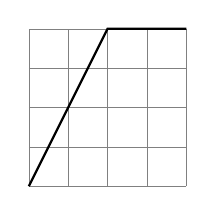
\begin{tikzpicture}
      \draw[step=0.5cm,gray,very thin] (0,0) grid (2,2);
      \draw[thick] (0,0) -- (1,2) -- (2,2);
    \end{tikzpicture}
    \quad
    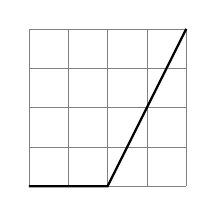
\begin{tikzpicture}
      \draw[step=0.5cm,gray,very thin] (0,0) grid (2,2);
      \draw[thick] (0,0) -- (1,0) -- (2,2);
    \end{tikzpicture}
    \quad
    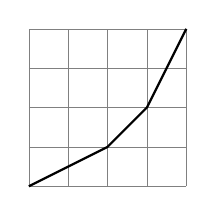
\begin{tikzpicture}
      \draw[step=0.5cm,gray,very thin] (0,0) grid (2,2);
      \draw[thick] (0,0) -- (1,0.5) -- (1.5,1) -- (2,2);
    \end{tikzpicture}
    \caption{Graphs of the functions $\phi_1$, $\phi_2$, and $\phi_3$ respectively.}
    \label{graph-reparametrisation}
  \end{figure}
  
  For (iii) we give a homotopy explicitly. Let us show that $\gamma \star \gamma^\inv \sim_p e_x$. For $t \in [0,1]$, define a path $\gamma_t : [0,1] \to X$ by $\gamma(s) = \gamma(ts)$, and define $G : [0,1] \times [0,1] \to X$ by
  \[
    G(s,t) = (\gamma_t \star \gamma_t^\inv)(s).
  \]
  That $G$ is continuous follows once again from an argument using Remark~\ref{pasting-closed}, and we see that $G$ is a homotopy from $e_x$ to $\gamma \star \gamma^\inv$ since
  \begin{align*}
    G(s,0) &= (\gamma_0 \star \gamma_0^\inv)(s) = \gamma(0) = x = e_x(s),\\
    G(s,1) &= (\gamma_1 \star \gamma_1^\inv)(s) = (\gamma \star \gamma^\inv)(s),\\
    G(0,t) &= \gamma_t(0) = \gamma(0) = x,\\
    G(1,t) &= \gamma_t^\inv(1) = \gamma(0) = x,
  \end{align*}
  for every $s$ and $t$. That $\gamma^\inv \star \gamma \sim_p e_y$ follows by an analogous argument.
\end{proof}


\subsection{The fundamental group}

\subsection{Covering spaces and examples}
